% Options for packages loaded elsewhere
\PassOptionsToPackage{unicode}{hyperref}
\PassOptionsToPackage{hyphens}{url}
%
\documentclass[
  man,floatsintext]{apa6}
\usepackage{amsmath,amssymb}
\usepackage{iftex}
\ifPDFTeX
  \usepackage[T1]{fontenc}
  \usepackage[utf8]{inputenc}
  \usepackage{textcomp} % provide euro and other symbols
\else % if luatex or xetex
  \usepackage{unicode-math} % this also loads fontspec
  \defaultfontfeatures{Scale=MatchLowercase}
  \defaultfontfeatures[\rmfamily]{Ligatures=TeX,Scale=1}
\fi
\usepackage{lmodern}
\ifPDFTeX\else
  % xetex/luatex font selection
\fi
% Use upquote if available, for straight quotes in verbatim environments
\IfFileExists{upquote.sty}{\usepackage{upquote}}{}
\IfFileExists{microtype.sty}{% use microtype if available
  \usepackage[]{microtype}
  \UseMicrotypeSet[protrusion]{basicmath} % disable protrusion for tt fonts
}{}
\makeatletter
\@ifundefined{KOMAClassName}{% if non-KOMA class
  \IfFileExists{parskip.sty}{%
    \usepackage{parskip}
  }{% else
    \setlength{\parindent}{0pt}
    \setlength{\parskip}{6pt plus 2pt minus 1pt}}
}{% if KOMA class
  \KOMAoptions{parskip=half}}
\makeatother
\usepackage{xcolor}
\usepackage{graphicx}
\makeatletter
\def\maxwidth{\ifdim\Gin@nat@width>\linewidth\linewidth\else\Gin@nat@width\fi}
\def\maxheight{\ifdim\Gin@nat@height>\textheight\textheight\else\Gin@nat@height\fi}
\makeatother
% Scale images if necessary, so that they will not overflow the page
% margins by default, and it is still possible to overwrite the defaults
% using explicit options in \includegraphics[width, height, ...]{}
\setkeys{Gin}{width=\maxwidth,height=\maxheight,keepaspectratio}
% Set default figure placement to htbp
\makeatletter
\def\fps@figure{htbp}
\makeatother
\setlength{\emergencystretch}{3em} % prevent overfull lines
\providecommand{\tightlist}{%
  \setlength{\itemsep}{0pt}\setlength{\parskip}{0pt}}
\setcounter{secnumdepth}{-\maxdimen} % remove section numbering
% Make \paragraph and \subparagraph free-standing
\ifx\paragraph\undefined\else
  \let\oldparagraph\paragraph
  \renewcommand{\paragraph}[1]{\oldparagraph{#1}\mbox{}}
\fi
\ifx\subparagraph\undefined\else
  \let\oldsubparagraph\subparagraph
  \renewcommand{\subparagraph}[1]{\oldsubparagraph{#1}\mbox{}}
\fi
% definitions for citeproc citations
\NewDocumentCommand\citeproctext{}{}
\NewDocumentCommand\citeproc{mm}{%
  \begingroup\def\citeproctext{#2}\cite{#1}\endgroup}
\makeatletter
 % allow citations to break across lines
 \let\@cite@ofmt\@firstofone
 % avoid brackets around text for \cite:
 \def\@biblabel#1{}
 \def\@cite#1#2{{#1\if@tempswa , #2\fi}}
\makeatother
\newlength{\cslhangindent}
\setlength{\cslhangindent}{1.5em}
\newlength{\csllabelwidth}
\setlength{\csllabelwidth}{3em}
\newenvironment{CSLReferences}[2] % #1 hanging-indent, #2 entry-spacing
 {\begin{list}{}{%
  \setlength{\itemindent}{0pt}
  \setlength{\leftmargin}{0pt}
  \setlength{\parsep}{0pt}
  % turn on hanging indent if param 1 is 1
  \ifodd #1
   \setlength{\leftmargin}{\cslhangindent}
   \setlength{\itemindent}{-1\cslhangindent}
  \fi
  % set entry spacing
  \setlength{\itemsep}{#2\baselineskip}}}
 {\end{list}}
\usepackage{calc}
\newcommand{\CSLBlock}[1]{\hfill\break\parbox[t]{\linewidth}{\strut\ignorespaces#1\strut}}
\newcommand{\CSLLeftMargin}[1]{\parbox[t]{\csllabelwidth}{\strut#1\strut}}
\newcommand{\CSLRightInline}[1]{\parbox[t]{\linewidth - \csllabelwidth}{\strut#1\strut}}
\newcommand{\CSLIndent}[1]{\hspace{\cslhangindent}#1}
\ifLuaTeX
\usepackage[bidi=basic]{babel}
\else
\usepackage[bidi=default]{babel}
\fi
\babelprovide[main,import]{english}
% get rid of language-specific shorthands (see #6817):
\let\LanguageShortHands\languageshorthands
\def\languageshorthands#1{}
% Manuscript styling
\usepackage{upgreek}
\captionsetup{font=singlespacing,justification=justified}

% Table formatting
\usepackage{longtable}
\usepackage{lscape}
% \usepackage[counterclockwise]{rotating}   % Landscape page setup for large tables
\usepackage{multirow}		% Table styling
\usepackage{tabularx}		% Control Column width
\usepackage[flushleft]{threeparttable}	% Allows for three part tables with a specified notes section
\usepackage{threeparttablex}            % Lets threeparttable work with longtable

% Create new environments so endfloat can handle them
% \newenvironment{ltable}
%   {\begin{landscape}\centering\begin{threeparttable}}
%   {\end{threeparttable}\end{landscape}}
\newenvironment{lltable}{\begin{landscape}\centering\begin{ThreePartTable}}{\end{ThreePartTable}\end{landscape}}

% Enables adjusting longtable caption width to table width
% Solution found at http://golatex.de/longtable-mit-caption-so-breit-wie-die-tabelle-t15767.html
\makeatletter
\newcommand\LastLTentrywidth{1em}
\newlength\longtablewidth
\setlength{\longtablewidth}{1in}
\newcommand{\getlongtablewidth}{\begingroup \ifcsname LT@\roman{LT@tables}\endcsname \global\longtablewidth=0pt \renewcommand{\LT@entry}[2]{\global\advance\longtablewidth by ##2\relax\gdef\LastLTentrywidth{##2}}\@nameuse{LT@\roman{LT@tables}} \fi \endgroup}

% \setlength{\parindent}{0.5in}
% \setlength{\parskip}{0pt plus 0pt minus 0pt}

% Overwrite redefinition of paragraph and subparagraph by the default LaTeX template
% See https://github.com/crsh/papaja/issues/292
\makeatletter
\renewcommand{\paragraph}{\@startsection{paragraph}{4}{\parindent}%
  {0\baselineskip \@plus 0.2ex \@minus 0.2ex}%
  {-1em}%
  {\normalfont\normalsize\bfseries\itshape\typesectitle}}

\renewcommand{\subparagraph}[1]{\@startsection{subparagraph}{5}{1em}%
  {0\baselineskip \@plus 0.2ex \@minus 0.2ex}%
  {-\z@\relax}%
  {\normalfont\normalsize\itshape\hspace{\parindent}{#1}\textit{\addperi}}{\relax}}
\makeatother

\makeatletter
\usepackage{etoolbox}
\patchcmd{\maketitle}
  {\section{\normalfont\normalsize\abstractname}}
  {\section*{\normalfont\normalsize\abstractname}}
  {}{\typeout{Failed to patch abstract.}}
\patchcmd{\maketitle}
  {\section{\protect\normalfont{\@title}}}
  {\section*{\protect\normalfont{\@title}}}
  {}{\typeout{Failed to patch title.}}
\makeatother

\usepackage{xpatch}
\makeatletter
\xapptocmd\appendix
  {\xapptocmd\section
    {\addcontentsline{toc}{section}{\appendixname\ifoneappendix\else~\theappendix\fi\\: #1}}
    {}{\InnerPatchFailed}%
  }
{}{\PatchFailed}
\usepackage{lineno}

\linenumbers
\usepackage{csquotes}
\raggedbottom
\ifLuaTeX
  \usepackage{selnolig}  % disable illegal ligatures
\fi
\usepackage{bookmark}
\IfFileExists{xurl.sty}{\usepackage{xurl}}{} % add URL line breaks if available
\urlstyle{same}
\hypersetup{
  pdflang={en-EN},
  hidelinks,
  pdfcreator={LaTeX via pandoc}}

\author{\phantom{0}}
\date{}


\shorttitle{A tutorial on hazard analysis}

\affiliation{\phantom{0}}

\begin{document}

\renewcommand{\figurename}{Supplementary Figure}
\renewcommand{\tablename}{Supplemetentary Table}

\section{Supplemental Material}\label{supplemental-material}

\subsection{A. Definitions of discrete-time hazard, surivor, probability mass, and conditional accuracy functions}\label{a.-definitions-of-discrete-time-hazard-surivor-probability-mass-and-conditional-accuracy-functions}

The shape of a distribution of waiting times can be described in multiple ways (Luce, 1991). After dividing time in discrete, contiguous time bins indexed by t, let RT be a discrete random variable denoting the rank of the time bin in which a particular person's response occurs in a particular experimental condition.
Because waiting times can only increase, discrete-time EHA focuses on the discrete-time hazard function

\noindent h(t) = P(RT = t\textbar{} RT \(\geq\) t) \hfill  (1)

\noindent and the discrete-time survivor function

\noindent S(t) = P(RT \(>\) t) = {[}1-h(t){]}.{[}1-h(t-1){]}.{[}1-h(t-2){]}\ldots{[}1-h(1){]} \hfill  (2)

\noindent and not on the probability mass function

\noindent P(t) = P(RT = t) = h(t).S(t-1) \hfill  (3)

\noindent nor the cumulative distribution function

\noindent F(t) = P(RT \(\leq\) t) = 1-S(t) \hfill  (4)

The discrete-time hazard function of event occurrence gives you for each bin the probability that the event occurs (sometime) in that bin, given that the event has not occurred yet in previous bins. This conditionality in the definition of hazard is what makes the hazard function so diagnostic for studying event occurrence, as an event can physically not occur when it has already occurred before. While the discrete-time hazard function assesses the unique risk of event occurrence associated with each time bin, the discrete-time survivor function cumulates the bin-by-bin risks of event \emph{non}occurrence to obtain the probability that the event occurs afer bin t. The probability mass function cumulates the risk of event occurrence in bin t with the risks of event nonoccurrence in bins 1 to t-1. From equation 3 we find that hazard in bin t is equal to P(t)/S(t-1).

For two-choice RT data, the discrete-time hazard function can be extended with the discrete-time conditional accuracy function

\noindent ca(t) = P(correct \textbar{} RT = t) \hfill  (5)

\noindent which gives you for each bin the probability that a response is correct given that it is emitted in time bin t (Allison, 2010; Kantowitz \& Pachella, 2021; Wickelgren, 1977). The ca(t) function is also known as the micro-level speed-accuracy tradeoff (SAT) function.

The survivor function provides a context for the hazard function, as S(t-1) = P(RT \textgreater{} t-1) = P(RT \(\geq\) t) tells you on how many percent of the trials the estimate h(t) = P(RT = t\textbar{} RT \(\geq\) t) is based. The probability mass function provides a context for the conditional accuracy function, as P(t) = P(RT = t) tells you on how many percent of the trials the estimate ca(t) = P(correct \textbar{} RT = t) is based.

While psychological RT data is typically measured in small, continuous units (e.g., milliseconds), discrete-time EHA treats the RT data as interval-censored data, because it only uses the information that the response occurred sometime in a particular bin of time (x,y{]}: x \textless{} RT \(\leq\) y. If we want to use the exact event times, then we treat time as a continuous variable, and let RT be a continous random variable denoting a particular person's response time in a particular experimental condition. Continuous-time EHA does not focus on the cumulative distribution function F(t) = P(RT \(\leq\) t) and its derivative, the probability density function f(t) = F(t)', but on the survivor function S(t) = P(RT \(>\) t) and the hazard rate function \(\lambda\)(t) = f(t)/S(t). The hazard rate function gives you the instantaneous \emph{rate} of event occurrence at time point t, given that the event has not occurred yet.

\subsection{B. Custom functions for descriptive discrete-time hazard analysis}\label{b.-custom-functions-for-descriptive-discrete-time-hazard-analysis}

We defined 12 custom functions that we list here.

\begin{itemize}
\tightlist
\item
  censor(df,timeout,bin\_width) : divide the time segment (0,timeout{]} in bins, identify any right-censored observations, and determine the discrete RT (time bin rank)
\item
  ptb(df) : transform the person-trial data set to the person-trial-bin data set
\item
  setup\_lt(ptb) : set up a life table for each level of 1 independent variable
\item
  setup\_lt\_2IV(ptb) : set up a life table for each combination of levels of 2 independent variables
\item
  calc\_ca(df) : estimate the conditinal accuracies when there is 1 independent variable
\item
  calc\_ca\_2IV(df) : estimate the conditional accuraies when there are 2 independent variables
\item
  join\_lt\_ca(df1,df2) : add the ca(t) estimates to the life tables (1 independent variable)
\item
  join\_lt\_ca\_2IV(df1, df2) : add the ca(t) estimates to the life tables (2 independent variables)
\item
  extract\_median(df) : estimate quantiles S(t)\textsubscript{.50} (1 independent variable)
\item
  extract\_median\_2IV(df) : estimate quantiles S(t)\textsubscript{.50} (2 independent variables)
\item
  plot\_eha(df, subj, haz\_yaxis=1, first\_bin\_shown=1, aggregated\_data=F, Nsubj=6) : create plots of the discrete-time functions (1 independent variable), and specify the upper limit of the y-axis in the hazard plot, with which bin to start plotting, whether the data is aggregated across participants, and across how many participants
\item
  plot\_eha\_2IV(df, subj, haz\_yaxis=1, first\_bin\_shown=1, aggregated\_data=F, Nsubj=6) : create plots of the discrete-time functions (2 independent variables), and specify the upper limit of the y-axis in the hazard plot, with which bin to start plotting, whether the data is aggregated across participants, and across how many participants
\end{itemize}

When you want to analyse simple RT data from a detection experiment with one independent variable, the functions calc\_ca() and join\_lt\_ca() should not be used, and the code to plot the conditional accuracy functions should be removed from the function plot\_eha().
When you want to analyse simple RT data from a detection experiment with two independent variables, the functions calc\_ca\_2IV() and join\_lt\_ca\_2IV() should not be used, and the code to plot the conditional accuracy functions should be removed from the function plot\_eha\_2IV().

\subsection{C. Link functions}\label{c.-link-functions}

Popular link functions include the logit link and the complementary log-log link, as shown in Supplementary Figure 1.



\begin{figure}[H]

{\centering 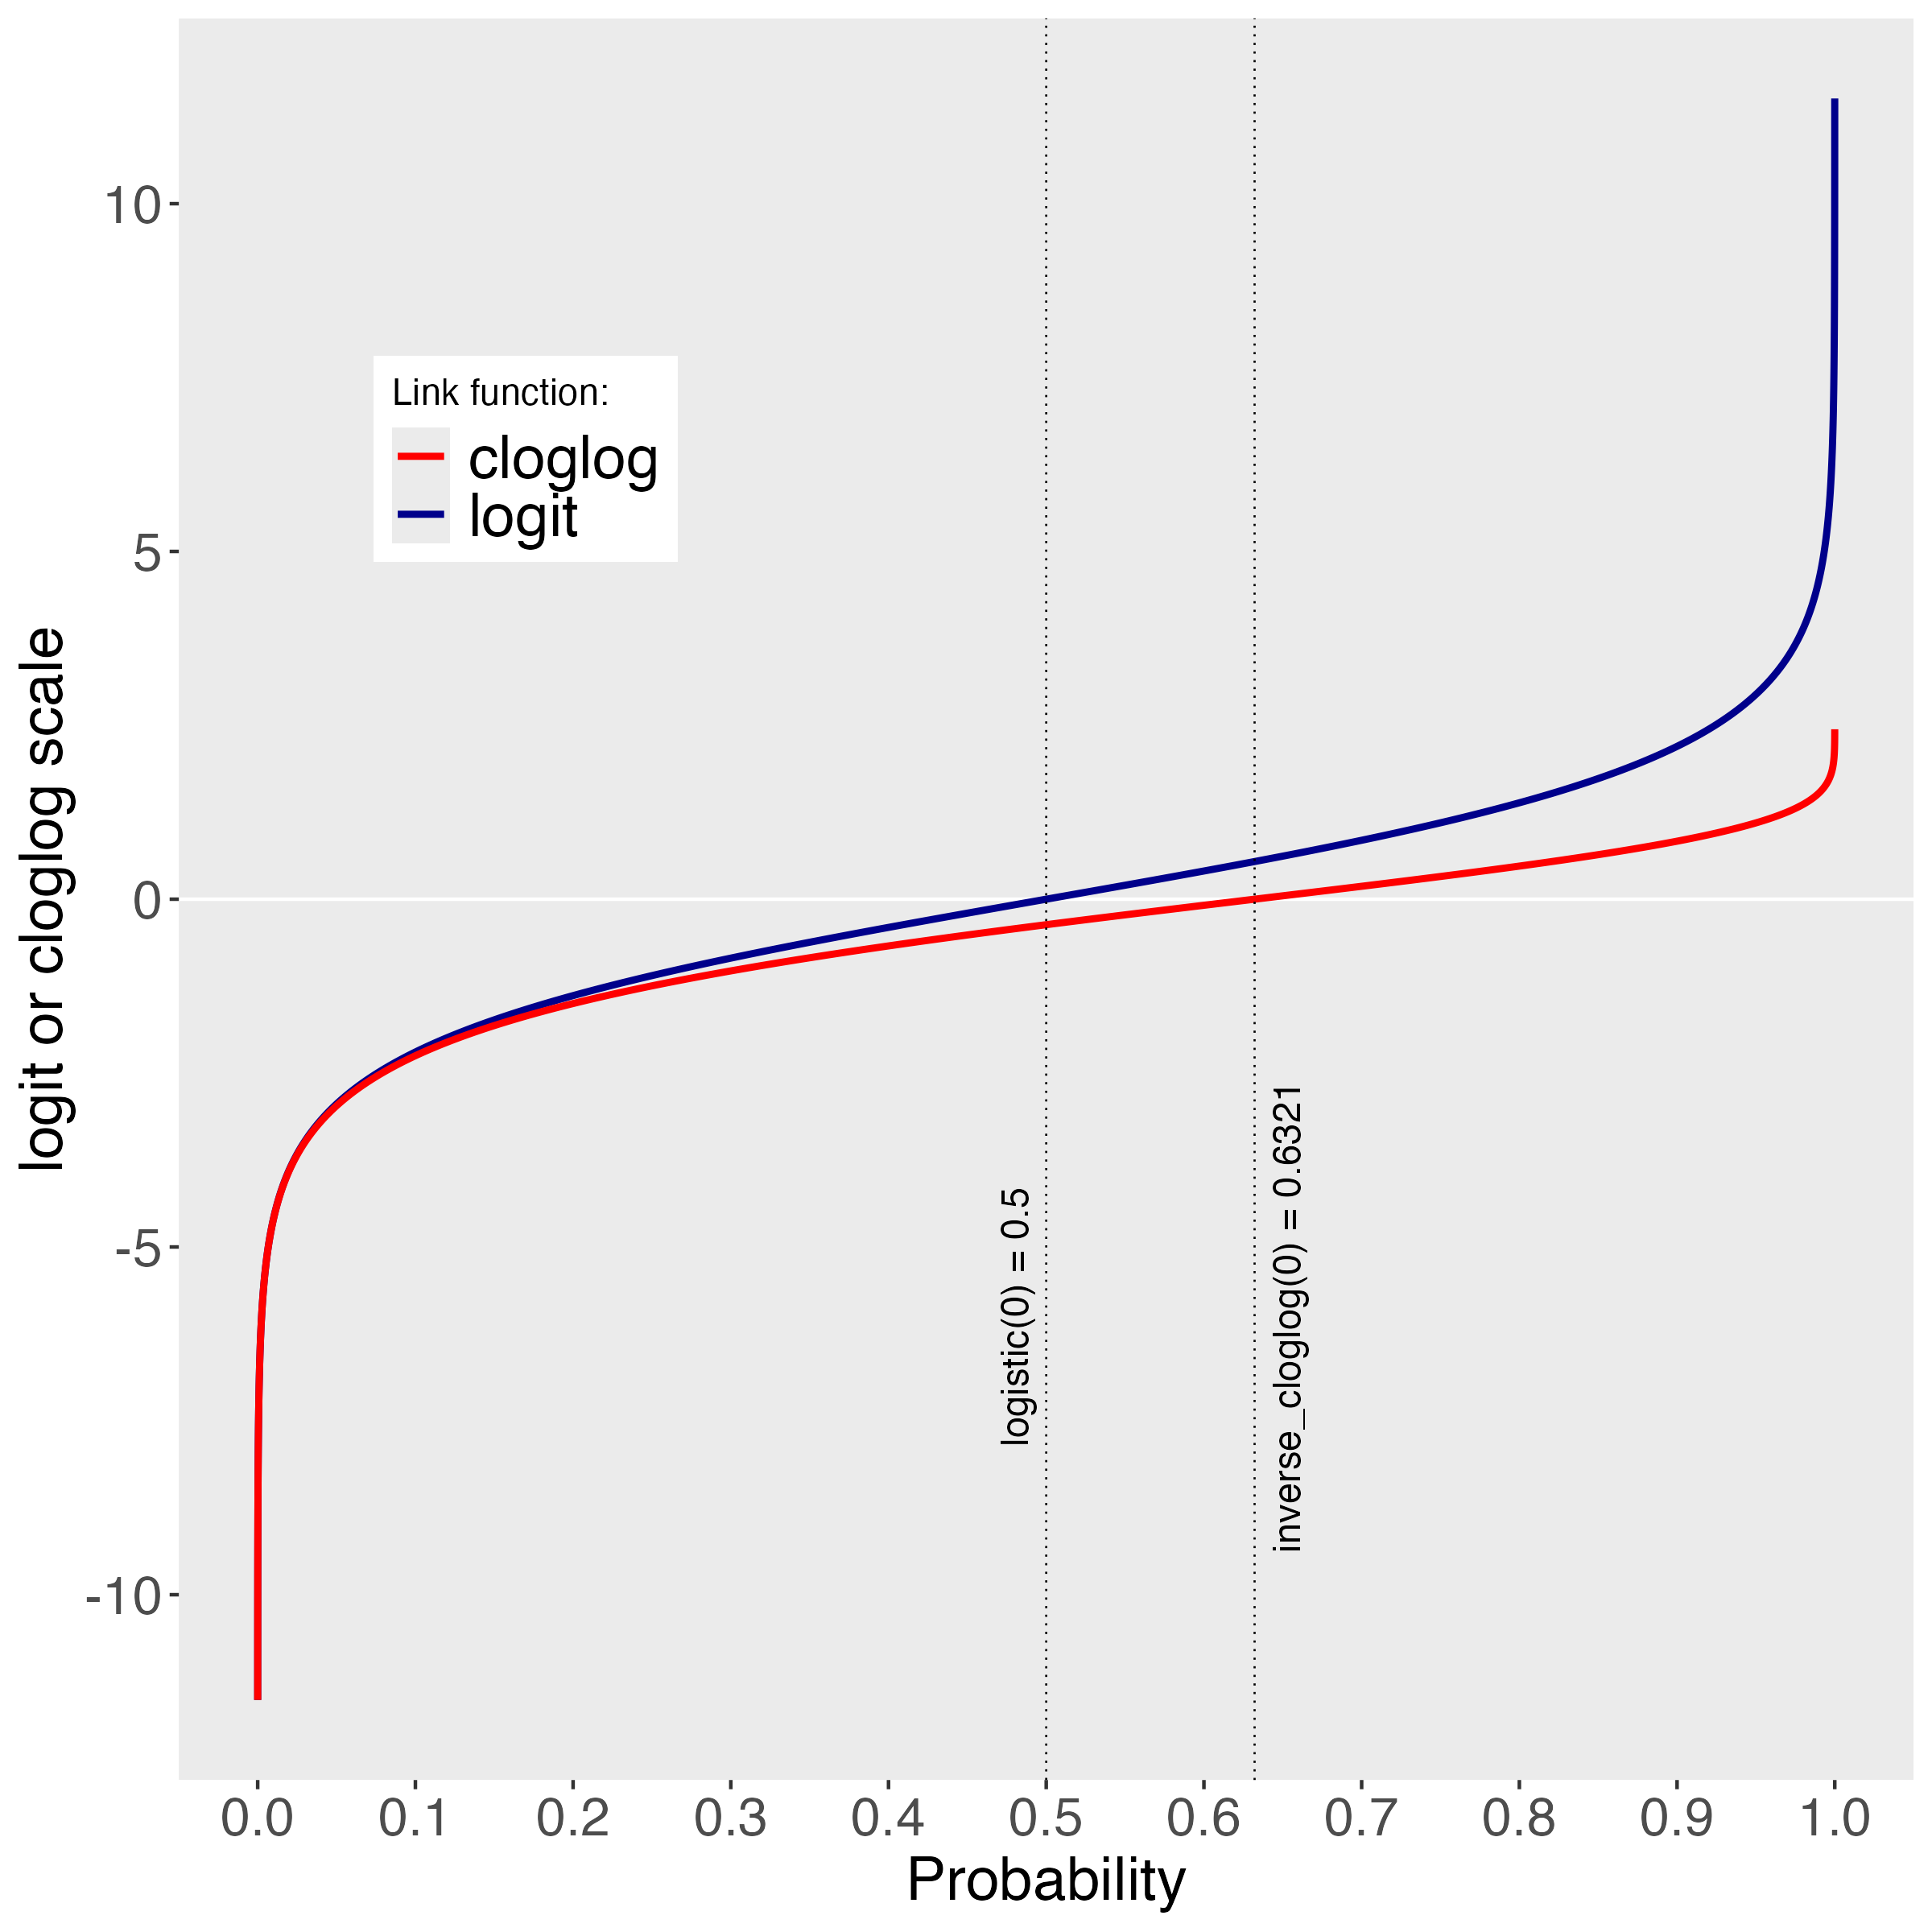
\includegraphics[width=0.8\linewidth,height=0.67\textheight,]{../../Tutorial_2_Bayesian/figures/linkfunctions} 

}

\caption{The logit and cloglog link functions.}\label{fig:plot-link-functions}
\end{figure}

\subsection{D. Regression equations}\label{d.-regression-equations}

An example (single-level) discrete-time hazard model with three predictors (TIME, X\textsubscript{1}, X\textsubscript{2}), the cloglog link function, and a second-order polynomial specification for TIME can be written as follows:

\noindent cloglog{[}h(t){]} = ln(-ln{[}1-h(t){]}) = {[}\(\beta\)\textsubscript{0}ONE + \(\beta\)\textsubscript{1}(TIME-9) + \(\beta\)\textsubscript{2}(TIME-9)\(^2\){]} + {[}\(\beta\)\textsubscript{3}X\textsubscript{1} + \(\beta\)\textsubscript{4}X\textsubscript{2} + \(\beta\)\textsubscript{5}X\textsubscript{2}(TIME-9){]} \hfill  (6)

The main predictor variable TIME is the time bin index t that is centered on value 9 in this example. The first set of terms within brackets, the parameters \(\beta\)\textsubscript{0} to \(\beta\)\textsubscript{2} multiplied by their polynomial specifications of (centered) time, represents the shape of the baseline cloglog-hazard function (i.e., when all predictors X\textsubscript{i} take on a value of zero). The second set of terms (the beta parameters \(\beta\)\textsubscript{3} to \(\beta\)\textsubscript{5}) represents the vertical shift in the baseline cloglog-hazard for a 1 unit increase in the respective predictor variable. Predictors can be discrete, continuous, and time-varying or time-invariant. For example, the effect of a 1 unit increase in X\textsubscript{1} is to vertically shift the whole baseline cloglog-hazard function by \(\beta\)\textsubscript{3} cloglog-hazard units. However, if the predictor interacts linearly with TIME (see X\textsubscript{2} in the example), then the effect of a 1 unit increase in X\textsubscript{2} is to vertically shift the predicted cloglog-hazard in bin 9 by \(\beta\)\textsubscript{4} cloglog-hazard units (when TIME-9 = 0), in bin 10 by \(\beta\)\textsubscript{4} + \(\beta\)\textsubscript{5} cloglog-hazard units (when TIME-9 = 1), and so forth. To interpret the effects of a predictor, its \(\beta\) parameter is exponentiated, resulting in a hazard ratio (due to the use of the cloglog link). When using the logit link, exponentiating a \(\beta\) parameter results in an odds ratio.

An example (single-level) discrete-time hazard model with a general specification for TIME (separate intercepts for each of six bins, where D1 to D6 are binary indicator variables identifying each bin) and a single predictor (X\textsubscript{1}) can be written as follows:

\noindent cloglog{[}h(t){]} = {[}\(\beta\)\textsubscript{0}D1 + \(\beta\)\textsubscript{1}D2 + \(\beta\)\textsubscript{2}D3 + \(\beta\)\textsubscript{3}D4 + \(\beta\)\textsubscript{4}D5 + \(\beta\)\textsubscript{5}D6{]} + {[}\(\beta\)\textsubscript{6}X\textsubscript{1}{]} \hfill  (7)

\subsection{E. Prior distributions}\label{e.-prior-distributions}

To gain a sense of what prior \emph{logit} values would approximate a uniform distribution on the probability scale, Kurz (2023) simulated a large number of draws from the Uniform(0,1) distribution, converted those draws to the log-odds metric, and fitted a Student's t distribution. Row C in Supplementary Figure 2 shows that using a t-distribution with 7.61 degrees of freedom and a scale parameter of 1.57 as a prior on the logit scale, approximates a uniform distribution on the probability scale. According to Kurz (2023), such a prior might be a good prior for the intercept(s) in a logit-hazard model, while the N(0,1) prior in row D might be a good prior for the non-intercept parameters in a logit-hazard model, as it gently regularizes p towards .5 (i.e., a zero effect on the logit scale).



\begin{figure}[H]

{\centering 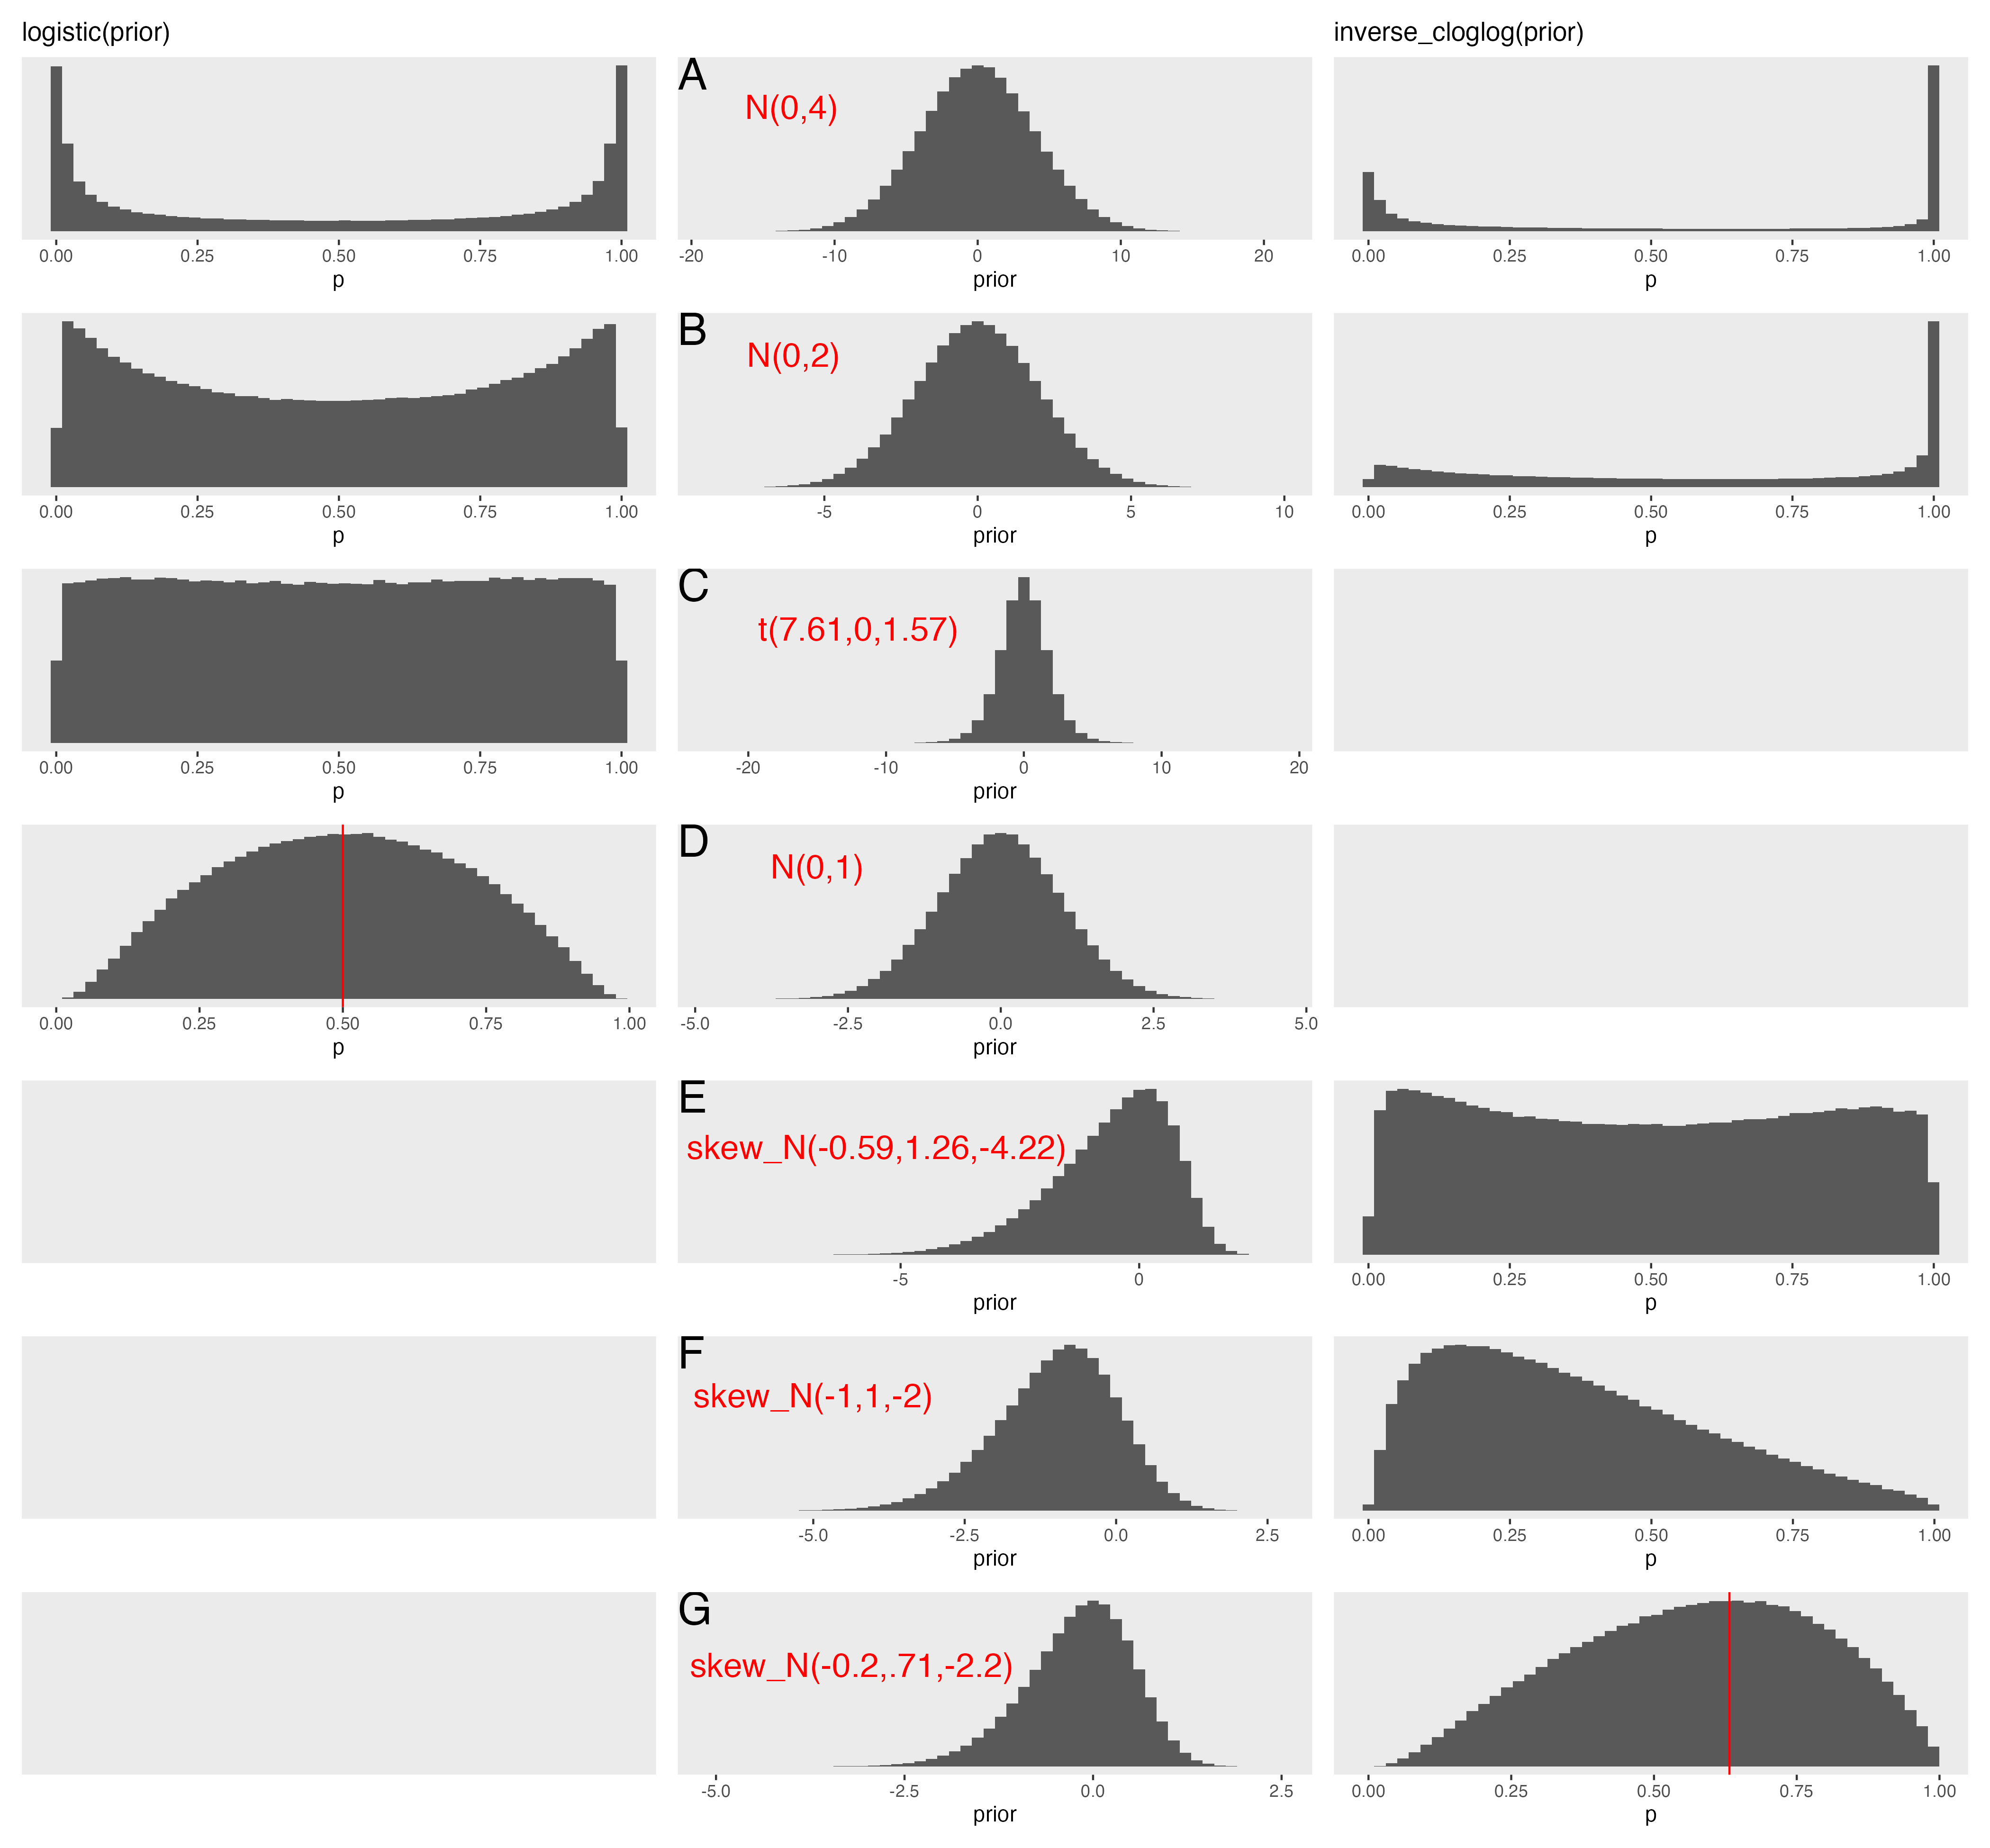
\includegraphics[width=0.8\linewidth,height=0.67\textheight,]{../../Tutorial_2_Bayesian/figures/plot_of_priors} 

}

\caption{Prior distributions for the Intercept on the logit and/or cloglog scales (middle column), and their implications on the probability scale after applying the inverse-logit (or logistic) transformation (left column), and the inverse-cloglog transformation (right column).}\label{fig:plot-priors}
\end{figure}

To gain a sense of what prior \emph{cloglog} values would approximate a uniform distribution on the hazard probability scale, we followed Kurz's approach and simulated a large number of draws from the Uniform(0,1) distribution, converted them to the cloglog metric, and fitted a skew-normal model (due to the asymmetry of the cloglog link function). Row E shows that using a skew-normal distribution with a mean of -0.59, a standard deviation of 1.26, and a skewness of -4.22 as a prior on the cloglog scale, approximates a uniform distribution on the probability scale.
However, because hazard values below .5 are more likely in RT studies, using a skew-normal distribution with a mean of -1, a standard deviation of 1, and a skewness of -2 as a prior on the cloglog scale (row F), might be a good weakly informative prior for the intercept(s) in a cloglog-hazard model.

\subsection{F. Advantages of hazard analysis}\label{f.-advantages-of-hazard-analysis}

Statisticians and mathematical psychologists recommend focusing on the hazard function when analyzing time-to-event data for various reasons. First, as discussed by Holden, Van Orden, and Turvey (2009), ``probability density {[}and mass{]} functions can appear nearly identical, both statistically and to the naked eye, and yet are clearly different on the basis of their hazard functions (but not vice versa). Hazard functions are thus more diagnostic than density functions'' (p.~331) when one is interested in studying the detailed shape of a RT distribution (see also Figure 1 in Panis, Schmidt, Wolkersdorfer, \& Schmidt, 2020). Therefore, when the goal is to study how psychological effects change over time, hazard and conditional accuracy functions are the preferred ways to describe the RT + accuracy data.

Second, because RT distributions may differ from one another in multiple ways, Townsend (1990) developed a dominance hierarchy of statistical differences between two arbitrary distributions A and B. For example, if h\textsubscript{A}(t) \textgreater{} h\textsubscript{B}(t) for all t, then both hazard functions are said to show a complete ordering. Townsend (1990) concluded that stronger conclusions can be drawn from data when comparing the hazard functions using EHA. For example, when mean A \textless{} mean B, the hazard functions might show a complete ordering (i.e., for all t), a partial ordering (e.g., only for t \textgreater{} 300 ms, or only for t \textless{} 500 ms), or they may cross each other one or more times.

Third, EHA does not discard right-censored observations when estimating hazard functions, that is, trials for which we do not observe a response during the data collection period in a trial so that we only know that the RT must be larger than some value (e.g., the response deadline). This is important because although a few right-censored observations are inevitable in most RT tasks, a lot of right-censored observations are expected in experiments on masking, the attentional blink, and so forth. In other words, by using EHA you can analyze RT data from experiments that typically do not measure response times. As a result, EHA can also deal with long RTs in experiments without a response deadline, which are typically treated as outliers and are discarded before calculating a mean. This orthodox procedure leads to underestimation of the true mean. By introducing a fixed censoring time for all trials at the end of the analysis time window, trials with long RTs are not discarded but contribute to the risk set of each bin.

Fourth, hazard modeling allows incorporating time-varying explanatory covariates such as heart rate, electroencephalogram (EEG) signal amplitude, gaze location, etc. (Allison, 2010). This is useful for linking physiological effects to behavioral effects when performing cognitive psychophysiology (Meyer, Osman, Irwin, \& Yantis, 1988).

Finally, as explained by Kelso, Dumas, and Tognoli (2013), it is crucial to first have a precise description of the macroscopic behavior of a system (here: h(t) and possibly ca(t) functions) in order to know what to derive on the microscopic level. EHA can thus solve the problem of model mimicry, i.e., the fact that different computational models can often predict the same mean RTs as observed in the empirical data, but not necessarily the detailed shapes of the empirical RT hazard distributions. Also, fitting parametric functions or computational models to data without studying the shape of the empirical discrete-time h(t) and ca(t) functions can miss important features in the data (Panis, Moran, Wolkersdorfer, \& Schmidt, 2020; Panis \& Schmidt, 2016).

\section*{References}\label{references}
\addcontentsline{toc}{section}{References}

\phantomsection\label{refs}
\begin{CSLReferences}{1}{0}
\bibitem[\citeproctext]{ref-allisonSurvivalAnalysisUsing2010}
Allison, P. D. (2010). \emph{Survival analysis using {SAS}: A practical guide} (2. ed). Cary, NC: SAS Press.

\bibitem[\citeproctext]{ref-holdenDispersionResponseTimes2009}
Holden, J. G., Van Orden, G. C., \& Turvey, M. T. (2009). Dispersion of response times reveals cognitive dynamics. \emph{Psychological Review}, \emph{116}(2), 318--342. \url{https://doi.org/10.1037/a0014849}

\bibitem[\citeproctext]{ref-kantowitzInterpretationReactionTime2021}
Kantowitz, B. H., \& Pachella, R. G. (2021). The {Interpretation} of {Reaction Time} in {Information-Processing Research} 1. \emph{Human Information Processing}, 41--82. \url{https://doi.org/10.4324/9781003176688-2}

\bibitem[\citeproctext]{ref-kelsoOutlineGeneralTheory2013}
Kelso, J. A. S., Dumas, G., \& Tognoli, E. (2013). Outline of a general theory of behavior and brain coordination. \emph{Neural Networks: The Official Journal of the International Neural Network Society}, \emph{37}, 120--131. \url{https://doi.org/10.1016/j.neunet.2012.09.003}

\bibitem[\citeproctext]{ref-kurzAppliedLongitudinalDataAnalysis2023}
Kurz, A. S. (2023). \emph{Applied longitudinal data analysis in brms and the tidyverse} (version 0.0.3). Retrieved from \url{https://bookdown.org/content/4253/}

\bibitem[\citeproctext]{ref-luceResponseTimesTheir1991}
Luce, R. D. (1991). \emph{Response times: Their role in inferring elementary mental organization} (1. issued as paperback). Oxford: Univ. Press.

\bibitem[\citeproctext]{ref-meyerModernMentalChronometry1988}
Meyer, D. E., Osman, A. M., Irwin, D. E., \& Yantis, S. (1988). Modern mental chronometry. \emph{Biological Psychology}, \emph{26}(1-3), 3--67. \url{https://doi.org/10.1016/0301-0511(88)90013-0}

\bibitem[\citeproctext]{ref-panisStudyingDynamicsVisual2020}
Panis, S., Moran, R., Wolkersdorfer, M. P., \& Schmidt, T. (2020). Studying the dynamics of visual search behavior using {RT} hazard and micro-level speed--accuracy tradeoff functions: {A} role for recurrent object recognition and cognitive control processes. \emph{Attention, Perception, \& Psychophysics}, \emph{82}(2), 689--714. \url{https://doi.org/10.3758/s13414-019-01897-z}

\bibitem[\citeproctext]{ref-panisAnalyzingResponseTimes2020}
Panis, S., Schmidt, F., Wolkersdorfer, M. P., \& Schmidt, T. (2020). Analyzing {Response Times} and {Other Types} of {Time-to-Event Data Using Event History Analysis}: {A Tool} for {Mental Chronometry} and {Cognitive Psychophysiology}. \emph{I-Perception}, \emph{11}(6), 2041669520978673. \url{https://doi.org/10.1177/2041669520978673}

\bibitem[\citeproctext]{ref-panisWhatShapingRT2016}
Panis, S., \& Schmidt, T. (2016). What {Is Shaping RT} and {Accuracy Distributions}? {Active} and {Selective Response Inhibition Causes} the {Negative Compatibility Effect}. \emph{Journal of Cognitive Neuroscience}, \emph{28}(11), 1651--1671. \url{https://doi.org/10.1162/jocn_a_00998}

\bibitem[\citeproctext]{ref-townsendTruthConsequencesOrdinal1990}
Townsend, J. T. (1990). Truth and consequences of ordinal differences in statistical distributions: {Toward} a theory of hierarchical inference. \emph{Psychological Bulletin}, \emph{108}(3), 551--567. \url{https://doi.org/10.1037/0033-2909.108.3.551}

\bibitem[\citeproctext]{ref-wickelgrenSpeedaccuracyTradeoffInformation1977}
Wickelgren, W. A. (1977). Speed-accuracy tradeoff and information processing dynamics. \emph{Acta Psychologica}, \emph{41}(1), 67--85. \url{https://doi.org/10.1016/0001-6918(77)90012-9}

\end{CSLReferences}


\end{document}
